\documentclass[11pt]{article}

\usepackage[margin=1in]{geometry}
\usepackage[T1]{fontenc}
\usepackage{lmodern}
\usepackage{listings}
\usepackage{xcolor}
\usepackage{enumitem}
\usepackage{setspace}
\usepackage{graphicx}
\usepackage{booktabs}

% hyperref should be loaded last
\usepackage{hyperref}

\graphicspath{{../screenshots/}}

\makeatletter
\newcommand{\annexlabel}[2]{%
  \phantomsection
  \def\@currentlabel{#2}%
  \label{#1}}
\makeatother

\lstset{
  basicstyle=\ttfamily\small,
  breaklines=true,
  columns=fullflexible,
  frame=single,
  backgroundcolor=\color{gray!10},
  keywordstyle=\color{blue!70!black},
  commentstyle=\color{green!50!black},
  stringstyle=\color{red!60!black},
  showstringspaces=false,
  numbers=left,
  numberstyle=\tiny\color{gray!70!black},
  xleftmargin=2em,
  captionpos=b,
}

\hypersetup{
  colorlinks=true,
  linkcolor=blue!60!black,
  urlcolor=blue!60!black,
  citecolor=blue!60!black,
  pdftitle={mboot: An Operating System Written from Scratch to Run Lua 5.5.0},
}

% Tolerate long unbreakable tokens (\texttt{...}) without overfull boxes
\setlength{\emergencystretch}{3em}
\onehalfspacing

\title{\textbf{mboot: An Operating System Written from Scratch\\to Run Lua 5.5.0}\\[0.5em]}
\author{Theo Marcos\\[0.4em]
\large Supervised by Daniel Kessler}
\date{April 2026}

\begin{document}
\maketitle

\begin{abstract}
\noindent This report documents \texttt{mboot}, an operating system written
from scratch as my TM, whose goal was
to run the Lua 5.5.0 interpreter as a user program. Starting from a bare
BIOS boot, \texttt{mboot} implements a bootloader, protected-mode setup,
interrupt handling, physical memory management and paging, an ATA disk
driver, a read-only FAT16 filesystem, an ELF32 loader, a preemptive
round-robin scheduler with \texttt{fork}/\texttt{exec}/\texttt{waitpid}, a
minimal C library, and a small network stack. Lua 5.5.0 runs \texttt{unmodified} as a user
program and provides an interactive prompt on each of four virtual
terminals about 0.3 seconds after kernel initialization begins in QEMU. The
report describes the system architecture, the Lua integration, the most
significant bugs encountered along the way, and what I learned from the
project. Three annexes, placed at the front of the report so that
beginners are not left behind, introduce the x86 architecture from
first principles, list \texttt{mboot}'s memory map, and document its
system call interface; together they are the only prerequisites for the
main text.
\end{abstract}

\newpage

\tableofcontents
\section{Introduction}
\label{sec:intro}

\textbf{Back to the future.} Imagine we could travel back in time to 1993,
the year Lua was born, and land next to a brand-new PC: a 386 or 486,
maybe 4 MB of RAM, a hard disk measured in tens of megabytes, a VGA
screen. In our pocket we carry a CD-ROM containing \texttt{mboot}: a
disk image built in 2026, whose programs include the Lua 5.5.0
interpreter, code that will not exist for another 32 years. (A
CD-ROM, deliberately: the format was standardized in 1988 and every PC
of the era could read one. A USB flash drive would have been useless as
the USB standard was published in 1996, and flash drives did not arrive
until around 2000.) Could we really use our disc?

The hardware could run it; the software could not. Every
instruction Lua needs already exists in a 1993 PC. The 32-bit machine
that Lua's implementation leans on (32-bit integers and pointers, a
flat address space with room for a few megabytes) has been part of
x86 since the Intel 80386 of 1985 (Table~\ref{tab:chronology}); ATA
hard disks (1986), FAT filesystems (1984), VGA displays and PS/2
keyboards (1987) are all there. What is missing is everything around
the interpreter: an operating system to manage that hardware, and a C
library to satisfy Lua's calls to \texttt{malloc}, \texttt{printf}, and
\texttt{setjmp}. In 1993, the only practical choice on a PC would have
been MS-DOS plus a commercial C compiler, and without an operating
system underneath, a disc of 32-bit executables is a coaster. This
project builds the missing piece. \texttt{mboot} is a small operating
system, written from scratch, whose reason to exist is that a 2025
interpreter can run on bare x86 metal, which means that with a time
machine, and mboot's image copied onto that hard disk with whatever
tools the era had, a machine from 1993 could speak a language from
2025.

\begin{table}[htbp]
\centering
\caption{The chronology behind the thought experiment: everything
\texttt{mboot} needs existed well before Lua 5.5.0.}
\label{tab:chronology}
\begin{tabular}{@{}clp{7.3cm}@{}}
\toprule
\textbf{Year} & \textbf{Event} & \textbf{Why it matters here} \\
\midrule
1978 & Intel 8086 & The x86 instruction set begins \\
1981 & IBM PC, BIOS, MBR boot & The boot process \texttt{mboot} still uses \\
1984 & FAT16 appears (DOS 3.0) & The filesystem \texttt{mboot} reads \\
1985 & Intel 80386 & 32-bit protected mode, paging, rings: the architecture \texttt{mboot} targets \\
1986 & ATA (IDE) standard & The disk driver \texttt{mboot} speaks \\
1987 & VGA text mode, PS/2 keyboard & The console and input of \texttt{mboot} \\
1988 & ISO 9660 standardizes CD-ROM & The disc our time traveler carries \\
1993 & Lua 1.0 first runs (28 July, never public) & The year we travel to \\
1994 & Lua 1.1, first public release (8 July) & Lua becomes usable by the world \\
1995 & ELF specification 1.2 & The executable format \texttt{mboot} loads \\
1996 & USB 1.0 is published & Too late for a USB stick in the story \\
2025 & Lua 5.5.0 released (22 Dec) & The interpreter \texttt{mboot} runs \\
2025--26 & \texttt{mboot} is built & This project \\
\bottomrule
\end{tabular}
\end{table}

For my TM project, I decided to write an operating system from scratch. I have been
programming for about a decade, with a lot of embedded work along the way,
building the kinds of abstractions that most programs take for granted. I
wanted to understand x86 on a deeper level and to see what it really takes
to get a complicated program running, which is why I picked this project.

The specific goal I chose was to make my operating system capable of running
Lua 5.5.0. I initially wanted to build a ``real'' operating system, but I
quickly realized that a full modern OS is not realistic scope for a TM. I
needed a concrete, achievable target that would still force me to build
genuine OS infrastructure. Lua 5.5.0 was a natural choice: it is a small,
self-contained, widely used scripting language, and getting a language
runtime to execute is a far more meaningful milestone than simply getting a
kernel to print text to a screen. A language runtime needs memory
allocation, file I/O, a C library, a process to run in, and a working
interrupt and timer infrastructure. If I could run Lua, I would have built
most of an operating system.

The central challenge was: how could I go from a machine that had just
booted (with no memory manager, no filesystem, no scheduler, and no C
library) to an environment capable of loading and executing Lua 5.5.0?

\clearpage
\section*{Annex A: A primer on x86, from first principles}
\annexlabel{annex:x86}{A}
\addcontentsline{toc}{section}{Annex A: A primer on x86, from first principles}

This annex explains, for a reader who has never done any systems
programming, the hardware concepts the report assumes. It requires no
knowledge beyond basic programming and every section below relates the hardware back to ideas you
already use every day.

\subsection*{A translation guide of the vocabulary used in this document}

\begin{itemize}[nosep]
  \item Every \texttt{print} you have ever written ends as a request to
  the operating system. A system call (Section~A.5) is exactly that
  request, made by executing a special CPU instruction instead of calling
  an ordinary function.
  \item A process is to a thread what a whole separate Python
  interpreter is to two threads inside one: its own program with its own
  memory, sharing only the CPU.
  \item File descriptors (used throughout Annex~\ref{annex:syscalls}) are
  small integers standing for open files; CPython's file objects wrap
  one under the hood, with 0, 1, and 2 fixed for standard input, output,
  and error, exactly as in Python.
  \item The scheduler does for processes what your desktop already does
  for windows: give each a turn in rotation (round-robin).
  \item Paging is like every process owning a private dict that maps its
  own addresses onto physical memory, so two programs can use the same
  address without ever seeing each other's objects.
\end{itemize}

\subsection*{A.1 The CPU, registers, and the stack}

A processor executes instructions one after another; each instruction is
stored in memory as a few bytes (machine code). The CPU keeps a handful of
very fast slots called registers. On 32-bit x86 there are the
general-purpose ones \texttt{EAX}, \texttt{EBX}, \texttt{ECX},
\texttt{EDX}, \texttt{ESI}, \texttt{EDI}, \texttt{ESP}, \texttt{EBP}, plus
one special register, \texttt{EIP} (the instruction pointer), which holds
the address of the next instruction. Jumps, calls, and interrupts are the
only things that make \texttt{EIP} skip somewhere else. \texttt{ESP} points
to the stack, an area of memory that function calls use to store
return addresses and local variables (last thing in, first thing out),
the same kind of bookkeeping as the call stack you see in a Python
traceback, but done by the CPU in hardware.
Working in C at this level is natural because a C compiler maps variables
and calls almost directly onto registers and the stack, but the C
standard library (\texttt{malloc}, \texttt{printf}, \ldots) is
itself software that must already exist. Providing it is one of
\texttt{mboot}'s jobs.

\subsection*{A.2 Power-on: real mode and the BIOS}

When a PC switches on there is no operating system; the firmware, the
\textbf{BIOS}, takes over. It initializes the hardware, runs a quick
self-test, and then tries to boot: it reads the first 512 bytes of the
boot disk (the \textbf{MBR}, Master Boot Record) into RAM at address
\texttt{0x7C00} and jumps there. The CPU starts in real mode: a
compatibility mode inherited from the 8086 of 1978, in which the CPU acts
like a 16-bit machine that can only directly address about 1~MB of memory.
Real mode also gives programs access to the BIOS's own routines through
software interrupts: \texttt{int 0x10} prints characters,
\texttt{int 0x13} reads disk sectors, and so on. \texttt{mboot}'s stage-1
bootloader lives entirely in this world: it uses those BIOS services to
read the rest of the system off the disk before leaving real mode behind.

\subsection*{A.3 Protected mode, the GDT, and rings}

The Intel 80386 (1985) introduced protected mode: 32-bit addresses
(up to 4~GB), memory protection, and privilege levels. Two structures must
exist before the switch. The \textbf{GDT} (Global Descriptor Table)
describes memory segments; \texttt{mboot} uses flat segments that
span all of memory, so segmentation does nothing interesting, but the
CPU refuses to enter protected mode without it. The switch itself is three
steps: disable interrupts, load the GDT, set bit \texttt{PE} of control
register \texttt{CR0}; then a far jump is needed to load the new code
segment and flush the CPU's instruction pipeline. Protection comes in four
privilege rings: ring~0 is the kernel, ring~3 is user code.
\texttt{mboot} deliberately runs everything in ring~0: proper user mode
requires extra bookkeeping whenever the
CPU crosses between rings, including a \textbf{TSS} (Task State Segment)
that tells the CPU which stack to use when an interrupt arrives while the
kernel is running. I judged that bookkeeping out of scope for this
project (it is listed under Known limitations), and it is a trade-off
I would make again.

\subsection*{A.4 Paging: virtual memory}

In protected mode the addresses used by code (virtual addresses)
can differ from the real RAM addresses (physical addresses). Paging
is the hardware that performs the translation: the CPU splits each virtual
address into a page number and a small offset, and looks the page number up
in tables held in RAM. The physical address of the top table sits in
control register \texttt{CR3}. Each entry can point a 4~KiB page at any
physical page and carries flags (present, writable, user-accessible). The
386 also supports huge 4~MiB pages (the \textbf{PSE} feature),
which \texttt{mboot}'s kernel uses to map all of physical memory 1-to-1
with only 1024 entries, an identity map where every virtual
address equals the physical one, so the kernel can keep using ordinary
pointers. Each user process gets its own page directory, so two programs
see different memory at the same addresses and cannot corrupt each other.
The highest bit of \texttt{CR0} switches paging on; from that moment every
single address the CPU touches goes through the tables.

\subsection*{A.5 Interrupts, the PIC, the timer, and system calls}

The CPU can be interrupted at any moment. There are two kinds.
Exceptions are synchronous: the CPU itself reports a problem, like a
division by zero or access to a page that is not present. Hardware
interrupts are asynchronous: devices raise electrical lines when they need
attention; those lines are wired to the \textbf{PIC} (8259 interrupt
controller), which tells the CPU which interrupt fired. Both kinds are
set up through the \textbf{IDT} (Interrupt Descriptor Table), a table of
256 entries mapping vector numbers to handler functions, the interrupt
analogue of the GDT. The PIC's 15 usable lines overlap the exception
range, so \texttt{mboot} remaps them to vectors \texttt{0x20}--\texttt{0x2F}.
One device matters more than any other: the \textbf{PIT}, a timer chip
from 1982, which raises interrupt~0 roughly 1000 times a second in
\texttt{mboot}. That heartbeat is what allows the scheduler to preempt the
current task and run another. User programs talk to the kernel the same
way: they execute the instruction \texttt{int 0x80} with the wanted system
call number in \texttt{EAX} and arguments in the other registers
(Annex~\ref{annex:syscalls}).

\subsection*{A.6 Talking to hardware}

Devices are driven two ways. With memory-mapped I/O, a device's
registers appear at ordinary physical addresses. The e1000 network card
and the VGA text buffer at \texttt{0xB8000} work like this. With
port I/O, there is a separate 64K address space addressed by the
dedicated \texttt{in}/\texttt{out} instructions: the PIT, PIC, keyboard
controller, serial port, and disk drive live there. Disk data can be moved
by DMA (the device writes RAM by itself) or by PIO (the CPU copies each
word through ports); \texttt{mboot} uses PIO only: simple and slow, but
correct.
Devices are discovered by walking the \textbf{PCI} bus, which exposes each
card's identity (vendor and device IDs) and where its registers sit (Base
Address Registers).

\subsection*{A.7 Glossary of terms used in this report}

\begin{center}
\setlength{\tabcolsep}{6pt}
\begin{tabular}{@{}lp{10.6cm}@{}}
\toprule
\textbf{Term} & \textbf{Meaning} \\
\midrule
BIOS & Firmware that boots the PC and offers low-level services in real mode \\
MBR & Master Boot Record: the first 512 bytes of the disk; the first code to run \\
GDT & Global Descriptor Table: describes segments and privilege levels \\
IDT & Interrupt Descriptor Table: maps interrupt vectors to handlers \\
TSS & Task State Segment: holds the kernel stack pointer for ring transitions \\
PIC & 8259 interrupt controller: routes device interrupts to the CPU \\
PIT & 8253/8254 timer chip: the system's heartbeat \\
IRQ & One hardware interrupt line from a device \\
E820 & BIOS service that reports which RAM regions physically exist \\
A20 line & Address line that unlocks RAM above 1~MiB; must be enabled by hand \\
Paging & Hardware virtual memory; \texttt{CR3} holds the table root address \\
PSE & The 4~MiB ``huge page'' extension used by the kernel identity map \\
Ring 0 & The highest privilege level \\
PIO & Programmed I/O: the CPU copies device data through ports \\
LBA28 & A 28-bit disk addressing scheme (disks up to 128~GiB) \\
VGA text & The 80$\times$25 character screen, backed by memory at \texttt{0xB8000} \\
UART & Serial port (16550 chip); \texttt{mboot} writes its log there \\
ELF & The executable file format Linux uses, and the one \texttt{mboot} loads \\
Syscall & A request for a kernel service, via \texttt{int 0x80} \\
\bottomrule
\end{tabular}
\end{center}

\clearpage
\section*{Annex B: \texttt{mboot}'s memory map}
\annexlabel{annex:memory}{B}
\addcontentsline{toc}{section}{Annex B: mboot's memory map}

None of these addresses are arbitrary; each one is fixed by a piece of
code (\texttt{stage1/boot.asm}, \texttt{stage2/loader.c}, or
\texttt{link.ld}). Some values were cross-checked against a real boot log
in QEMU.

\begin{center}
\begin{tabular}{@{}llp{9.2cm}@{}}
\toprule
\textbf{Address} & \textbf{Set by} & \textbf{What lives there} \\
\midrule
\texttt{0x00000}--\texttt{0x004FF} & BIOS & Real-mode interrupt table and BIOS data (left untouched) \\
\texttt{0x7C00} & BIOS & Stage-1 bootloader (the 512-byte MBR) \\
\texttt{0x10000} & \texttt{link.ld} & Kernel image: code, constants, data, zeroed BSS \\
\texttt{0x70FF0} & stage 1 & Count of E820 memory-map entries (16-bit) \\
\texttt{0x71000} & stage 1 & The E820 memory map itself (read by the allocator) \\
\texttt{0x90000} & stage 1 & Initial stack, set when entering protected mode \\
\texttt{0xB8000} & hardware & VGA text framebuffer (80$\times$25 characters, 2 bytes each) \\
\texttt{0x100000}+ & E820 & Extended RAM; the heap uses the largest usable region \\
\texttt{0x105000} & kernel & Page directory (CR3), 4~KiB-aligned (example from a real boot) \\
\texttt{0xFEBC0000} & PCI/e1000 & Memory-mapped registers of the network card (BAR0) \\
\texttt{0x47000000}, \texttt{0x50000000} & ELF loader & Fixed base address per program (\texttt{getty}, \texttt{lua}; \texttt{lua.elf} occupies 159~KiB); every process gets its own isolated copy \\
above the image & scheduler & The 64~KiB user stack of each process \\
\bottomrule
\end{tabular}
\end{center}

The layout has two halves with very different histories: below about
1~MiB, the legacy real-mode world the BIOS set up when the machine
started (which is why the kernel sits at \texttt{0x10000}, safely above
the BIOS structures, since \texttt{0x1000}, its first home, was not); and the
high addresses near half a gigabyte, where user programs are linked and
isolated from each other by per-process page tables.

\clearpage
\section*{Annex C: System call reference}
\annexlabel{annex:syscalls}{C}
\addcontentsline{toc}{section}{Annex C: System call reference}

System calls are invoked with the instruction \texttt{int 0x80}: the
syscall number goes in \texttt{EAX}, arguments in \texttt{EBX},
\texttt{ECX}, \texttt{EDX}, \texttt{ESI}, \texttt{EDI} (the classic Linux
i386 convention), and the result comes back in \texttt{EAX}. The numbers
were borrowed from Linux where such a syscall exists (\texttt{exec} is
\texttt{execve}'s number), so familiar muscle memory transfers; the socket
calls start at 300 to leave room for future POSIX numbers.

\begin{center}
\setlength{\tabcolsep}{5pt}
\begin{tabular}{@{}clp{5.9cm}p{5.0cm}@{}}
\toprule
\textbf{\#} & \textbf{Name} & \textbf{Arguments} & \textbf{Returns} \\
\midrule
1 & \texttt{exit} & EBX = exit code & never returns \\
2 & \texttt{fork} & --- & 0 in the child, child's PID in the parent \\
3 & \texttt{read} & EBX = fd, ECX = buffer, EDX = count & bytes read, or $-1$ \\
4 & \texttt{write} & EBX = fd, ECX = buffer, EDX = count & bytes written (fd 1 is also mirrored to serial) \\
5 & \texttt{open} & EBX = path & file descriptor, or $-1$ \\
6 & \texttt{close} & EBX = fd & 0 (fds 0--2 cannot be closed) \\
7 & \texttt{waitpid} & EBX = child PID & child's exit code, or $-1$ \\
11 & \texttt{exec} & EBX = path, ECX = argv, EDX = argc, ESI = tty ($-1$ = current) & never returns on success, $-1$ on failure \\
54 & \texttt{ioctl} & EBX = fd, ECX = request, EDX = arg & result; only \texttt{TIOCSCTTY} is implemented \\
63 & \texttt{dup2} & EBX = old fd, ECX = new fd & new fd, or $-1$ \\
300 & \texttt{socket} & EBX = domain, ECX = type, EDX = protocol & file descriptor, or $-1$ \\
301 & \texttt{bind} & EBX = fd, ECX = address, EDX = length & 0, or $-1$ \\
302 & \texttt{sendto} & EBX = fd, ECX = buffer, EDX = length, ESI = destination, EDI = length & bytes sent, or $-1$ \\
303 & \texttt{recvfrom} & EBX = fd, ECX = buffer, EDX = length, ESI = source (out), EDI = pointer to length & bytes received, or $-1$ \\
\bottomrule
\end{tabular}
\end{center}

\section{Initial Idea and Goals}
\label{sec:goals}

I arrived at the idea after reading about OS development and looking at small hobby
kernels. I initially wanted to build something that could run user programs
and maybe a shell. After getting a few early demo programs of my own running
(small programs that showed the growing kernel could load a file from
disk and execute it) I realized that the most interesting and testable
goal was to run a real language runtime. I
chose Lua 5.5.0 specifically because it was the newest release at the time
(it came out on 22 December 2025), it is
designed to be embedded and portable, and its source tree is small enough to
read and understand. I also liked that Lua is used in real products (games,
embedded systems, web servers via OpenResty), so it was not a toy.

My original goals were:
\begin{enumerate}[nosep]
  \item Boot from BIOS into 32-bit protected mode.
  \item Set up a GDT, IDT, and basic interrupt handling.
  \item Implement memory management (paging and a heap allocator).
  \item Read files from a FAT16 disk.
  \item Load and run ELF executables.
  \item Provide a minimal C library for user programs.
  \item Build Lua 5.5.0 against that C library and run it.
\end{enumerate}

Goals that were added later, as the project grew, included a preemptive
scheduler with \texttt{fork}/\texttt{exec}/\texttt{waitpid}, a VFS (virtual
file system) layer (a single interface through which files, terminals,
and sockets all look like open files), multiple TTYs, a VGA text-mode
console, a serial port for logging, a PCI bus
driver, an Intel e1000 network driver, and a small TCP/IP-style network stack
(Ethernet, ARP, IPv4, ICMP, UDP). These were not part of the original plan;
they emerged because I wanted to see how far I could push the system and
because some of them (like a scheduler) were needed to run multiple Lua
processes.

The final implementation differs substantially from the original plan in
scope, but not in spirit. I did not set out to build a network stack or a
multi-TTY console. I set out to build a system that could run Lua, and
ended up building a small operating system around that goal that went
further than the plan ever did. Table~\ref{tab:goals} in Section~\ref{sec:results} maps each of
these original goals to its final outcome.

\section{Planning Process}
\label{sec:plan}

I planned the project as a dependency chain. An operating system is
layered, and each layer depends on the ones below it. The chain I followed
was roughly:

\begin{enumerate}[nosep]
  \item Get code executing (bootloader, protected mode).
  \item Establish the CPU environment (GDT, IDT, interrupts).
  \item Initialize memory (E820 map, heap allocator, paging).
  \item Initialize hardware and basic I/O (PIC, PIT, serial, VGA, keyboard).
  \item Load programs (ATA disk, FAT16, ELF loader).
  \item Provide the environment Lua needs (C library, syscalls, process).
  \item Build and integrate Lua.
  \item Execute Lua code.
\end{enumerate}

The git history shows this progression clearly. The first commit
(\texttt{9234416}, September 2025) was a bootloader project with a stage-1
MBR, a stage-2 loader, disk I/O, and serial output. Over the next few
months I added interrupt handling, a keyboard driver, a memory allocator,
paging, a FAT16 driver, a VFS layer, an ELF loader, and a syscall interface.
The scheduler was first attempted in September 2025
(\texttt{aa1d32a}), then removed (\texttt{2a0b759}, October 2025) because
it was buggy and I did not have time to fix it, and re-implemented from
scratch in July 2026 (\texttt{cca70b5}) once I had a better understanding
of what I needed (see Section~\ref{sec:blocking}).

My original plan changed in several important ways. I initially tried to
build the kernel as a position-independent executable (PIE)
(\texttt{e585177}, November 2025), but I dropped that plan in favor of
paging with a fixed load address (\texttt{8405dad}) because paging gave me
memory isolation and a simpler mental model. I also originally planned to
keep everything in the kernel, but I later moved the init system into
userspace (\texttt{ce6d919}, August 2026) so that user programs could manage
their own processes. The network stack was not planned at all; it appeared
in October 2025 (\texttt{03ddbb0}) as an experiment and grew into a
full IPv4/UDP/ICMP implementation.

For research, I relied on the sources listed in the References section and
in the repository's \texttt{SOURCES.md}. The
Intel 64 and IA-32 Software Developer's Manual was my normative reference
for CPU behavior (GDT, IDT, paging, TSS). The OSDev Wiki provided practical
guides for the boot process, the E820 memory map, the PIC, the PIT, and
ATA PIO mode. The Microsoft FAT specification and the ELF specification
were essential for the filesystem and loader. For networking, I read
RFC~791 (IP), RFC~826 (ARP), RFC~768 (UDP), and RFC~792 (ICMP), plus the
Intel e1000 datasheet. For Lua, I read the Lua 5.5 Reference Manual and the
Lua source itself.

\section{How the System Works}
\label{sec:arch}

This section uses the concepts introduced in
Annexes~\ref{annex:x86} and~\ref{annex:memory}, which sit at the front of
the report so that this part of the text can stay short. The boot flow from
power-on to Lua execution is:

\begin{lstlisting}[language={},caption={Boot flow from power-on to the Lua REPL},label={lst:bootflow}]
Machine starts (BIOS, 16-bit real mode)
      |
      v
stage1/boot.asm  (MBR @ 0x7C00)
  - save boot drive, clear screen
  - detect memory via int 0x15 E820
  - load kernel.bin sectors via int 0x13
  - enable A20, load GDT, enter protected mode
    (flat segments, stack at 0x90000)
      |
      v
stage2/start_loader.asm  (trampoline @ 0x10000)
  - jump straight into loader_start()
      |
      v
stage2/loader.c  (kernel init)
  - mask PIC, remap to 0x20/0x28, init IDT
  - install exception ISRs, init PIT (~1000 Hz)
  - enable FPU, init keyboard, serial, CPUID
  - init allocator from E820 map
  - init TTYs, enable 4 MiB identity paging
  - enumerate PCI, init network
  - init GDT + TSS, init scheduler
  - init FAT16, spawn /init.elf
      |
      v
userspace: init -> getty x4 -> lua.elf
\end{lstlisting}

The BIOS loads the first sector of the disk (the MBR) to physical address
\texttt{0x7C00} and jumps to it in 16-bit real mode. My stage-1 bootloader
(\texttt{stage1/boot.asm}) saves the boot drive number from \texttt{DL},
clears the screen with BIOS interrupt \texttt{0x10}, and calls the E820
memory detection routine (\texttt{int 0x15}, \texttt{EAX=0xE820}) to build a
memory map at \texttt{0x71000}. It then loads the kernel binary
(\texttt{kernel.bin}) from the sectors after the MBR using BIOS disk
services (\texttt{int 0x13}, \texttt{AH=0x02}), enables the A20 line via
port \texttt{0x92}, loads a small GDT, and switches to protected mode by
setting \texttt{CR0.PE}.

Entering protected mode, stage 1 already sets the segment registers to a
flat 32-bit data segment and puts the stack at \texttt{0x90000}; it then
calls the kernel image at \texttt{0x10000}, where the trampoline
(\texttt{stage2/start\_loader.asm}) jumps straight into
\texttt{loader\_start()} in \texttt{stage2/loader.c}. The kernel
initialization routine masks all PIC interrupts, remaps the 8259 PIC to
vectors \texttt{0x20}/\texttt{0x28}, initializes the IDT, installs
exception handlers, initializes the PIT (divisor 1193, roughly 1000~Hz),
enables the FPU, and sets up the keyboard and serial port. It then
initializes the heap allocator from the E820 map, initializes the TTY
layer, and enables 4 MiB identity paging. After that it enumerates PCI
devices, initializes the network interface, sets up the GDT with a TSS,
and initializes the scheduler. Finally it mounts the FAT16 filesystem and
spawns the first user program, \texttt{/init.elf}.

The disk image (\texttt{image.sh}) contains the boot binary in the first
partition and a FAT16 filesystem in the second partition. The FAT16
partition holds the user programs: \texttt{init.elf}, \texttt{getty.elf},
\texttt{lua.elf}, and various test programs. The \texttt{init} program
spawns \texttt{getty} on each of four TTYs. \texttt{Getty} is a small
program in the Unix tradition that opens a terminal and starts whatever
runs on it; in \texttt{mboot} it simply executes \texttt{lua.elf}, giving
a Lua REPL on each terminal. Four terminals running Lua at once,
switched with Alt+F1 through Alt+F4, are the most visible proof that the
scheduler really does preempt and rotate between processes
(Section~\ref{sec:sched}). Every important address in this layout (where
the bootloader sits, where the kernel is linked, where user programs
live) is collected in one table in Annex~\ref{annex:memory}.

\section{Interesting Parts of the Code}

\subsection{Bootloader: \texttt{stage1/boot.asm}}
\label{sec:boot}

The bootloader is the first code that runs, and it has to work in 16-bit
real mode with only 512 bytes. The most interesting part is the transition
to protected mode:

\begin{lstlisting}[language={[x86masm]Assembler},caption={Protected mode transition in stage1/boot.asm}]
switch_to_pm:
	cli
	in al, 0x92
	or al, 2
	out 0x92, al
	lgdt [gdt_descriptor]

	mov eax, cr0
	or eax, 0x1
	mov cr0, eax

	jmp CODE_SEG:init_pm
\end{lstlisting}

This sequence disables interrupts, enables the A20 line (which allows
access to memory above 1~MiB), loads the GDT, and sets the PE bit in
\texttt{CR0}. The far jump \texttt{jmp CODE\_SEG:init\_pm} is required to
flush the CPU pipeline and load the new code segment selector. I
encountered a bug here early on: the kernel load address conflicted with
other low-memory data and had to be moved
(Section~\ref{sec:loadaddr}).

\subsection{Linker script: \texttt{link.ld}}
\label{sec:linker}

The kernel is linked at a fixed physical address:

\begin{lstlisting}[language={},caption={link.ld}]
OUTPUT_FORMAT(elf32-i386)
ENTRY(_start)

SECTIONS
{
    . = 0x10000;

    .text : { *(.text*) }
    .rodata : { *(.rodata*) }
    .data : { *(.data*) }
    .bss : { *(.bss*) *(COMMON) }
}
\end{lstlisting}

I needed the kernel at a known address because the bootloader loads it to
\texttt{0x10000} and jumps there. The linker script itself is simple, but
getting the address right was not: the original link address at
\texttt{0x1000} caused real conflicts in low memory
(Section~\ref{sec:loadaddr}).

\subsection{Kernel initialization: \texttt{stage2/loader.c}}
\label{sec:loader}

The \texttt{loader\_start()} function is the heart of the kernel. It calls
initialization routines in dependency order:

\begin{lstlisting}[language=C,caption={Excerpt from loader.c}]
void loader_start(void) {
  for (int i = 0; i < IRQs; ++i) {
    pic_set_mask(i);
  }

  pic_remap();
  idt_init();
  install_exception_isrs();
  pit_init();
  enable_fpu();
  install_keyboard();
  init_serial();
  cpuid_init();

  e820_entry_t *mem_map = E820_TABLE_ADDR;
  uint16_t entry_count = *E820_ENTRY_COUNT_ADDR;
  init_alloc(entry_count, mem_map);
  tty_init();
  paging_init();

  pci_enumerate();
  net_init();
  gdt_init();
  scheduler_init();
  pic_clear_mask(0);
  install_irq(0, NULL);
  uint32_t esp;
  asm("mov %%esp, %0" : "=r"(esp));
  tss_set_stack(esp, GDT_DATA_SEG);

  fat16_init();

  char *argv[] = {"init", NULL};
  int argc = 1;

  INFO("MAIN", "Starting init...");
  if (spawn_elf("/init.elf", argc, argv, -1) < 0) {
    while (1) {
      asm volatile("hlt");
    }
  }

  STI();
  INFO("MAIN", "Init scheduled. Entering idle loop.");
  while (1) {
    asm volatile("hlt");
  }
}
\end{lstlisting}

The ordering here is deliberate. The PIC is masked first so that no
interrupts fire before the IDT is ready. The allocator is initialized from
the E820 map before paging is enabled, because paging needs to allocate a
page directory. The TSS stack is set just before \texttt{STI()} enables
interrupts, so that any interrupt arriving after that point finds a valid
kernel stack. The \texttt{install\_irq(0, NULL)}
call deliberately installs no user handler for the timer IRQ: the
interrupt dispatcher special-cases IRQ~0 and calls the scheduler's tick
function itself (Section~\ref{sec:sched}). The final \texttt{hlt} loop is
the idle task; it halts the CPU until the next interrupt.

\subsection{Memory allocator: \texttt{stage2/mem.c}}
\label{sec:mem}

I implemented a bump allocator with a free list. The allocator manages the
largest usable region from the E820 map. Each block has a header with a size
and a free flag:

\begin{lstlisting}[language=C,caption={Excerpt from mem.c: kmalloc}]
void *kmalloc(uint32_t bytes) {
  const uintptr_t ALIGN = 8;
  if (bytes == 0)
    return NULL;
  uintptr_t want_size = (uintptr_t)bytes;
  want_size = align_up_uintptr(want_size, ALIGN);

  if (bump_next == 0) {
    bump_next = free_ram;
  }

  block_header_t *found = find_free_block_and_remove((uint32_t)want_size);
  if (found) {
    try_split_block(found, (uint32_t)want_size);
    void *payload = (void *)((uintptr_t)found + sizeof(block_header_t));
    memset(payload, 0, want_size);
    return payload;
  }

  uintptr_t hdr_addr =
      align_up_uintptr(bump_next, ALIGN);
  uintptr_t payload_addr = hdr_addr + sizeof(block_header_t);
  uintptr_t new_bump = payload_addr + want_size;

  if (new_bump > free_ram_end) {
    ERROR("MEM", "Out of memory :(");
    HALT();
  }

  block_header_t *hdr = (block_header_t *)hdr_addr;
  hdr->size = (uint32_t)want_size;
  hdr->free = 0;
  hdr->next = NULL;

  bump_next = new_bump;

  void *payload = (void *)payload_addr;
  memset(payload, 0, want_size);
  return payload;
}
\end{lstlisting}

The kernel needs dynamic memory for task control
blocks, page tables, file buffers, and other data structures. The allocator
first tries to find a free block of sufficient size; if none is found, it
bumps the allocation pointer. When a block is freed, it is added back to
the free list and coalesced with adjacent free blocks. I encountered a bug
early on where the allocator did not align headers correctly, causing
memory corruption.

\subsection{Paging: \texttt{stage2/paging.c}}
\label{sec:paging}

I implemented 4 MiB identity paging for the kernel and 4 KiB paging for
user processes. The kernel page directory maps the first 4 GiB of physical
memory to the same virtual addresses using 4 MiB pages (enabled via
\texttt{CR4.PSE}):

\begin{lstlisting}[language=C,caption={Excerpt from paging.c: paging\_init}]
void paging_init(void) {
  uintptr_t raw_page_directory = (uintptr_t)kmalloc(PAGE_SIZE * 2);
  page_directory = (uint32_t *)align_up_uintptr(raw_page_directory, PAGE_SIZE);

  for (uint32_t i = 0; i < PAGE_DIRECTORY_ENTRIES; ++i) {
    uint32_t phys = i * FOUR_MIB;
    page_directory[i] =
        (phys & 0xFFC00000U) | PAGE_PRESENT | PAGE_WRITABLE | PAGE_SIZE_4MB;
  }

  write_cr4(read_cr4() | 0x00000010U);
  write_cr3((uint32_t)page_directory);
  write_cr0(read_cr0() | 0x80000000U);

  INFO("PAGING", "Enabled 4 MiB identity paging (CR3=0x%X)", read_cr3());
}
\end{lstlisting}

I needed paging to give each user process its own address space. The
\texttt{paging\_map\_page} function splits a 4 MiB page into 4 KiB pages
when a user process needs finer-grained mapping; this was the source of one
of my nastiest bugs (Section~\ref{sec:pagebug}).

\subsection{ELF loader: \texttt{stage2/elf.c}}
\label{sec:elfloader}

The ELF loader reads an executable from the FAT16 filesystem, parses its
program headers, and creates a user task:

\begin{lstlisting}[language=C,caption={Excerpt from elf.c: spawn\_elf}]
int spawn_elf(const char *path, int argc, char **argv, int tty) {
  int file = file_open(path);
  if (file < 0) {
    INFO("ELF", "error: could not find %s", path);
    return -1;
  }

  int size = fat16_get_size(file);
  void *buf = kmalloc(size);
  file_read(file, size, buf);
  file_close(file);

  INFO("ELF", "%s loaded (%d bytes)", path, size);
  Elf32_Ehdr *eh = (Elf32_Ehdr *)buf;
  if (eh->magic != ELF_MAGIC) {
    INFO("ELF", "error: %s is not a valid ELF", path);
    return -1;
  }

  user_segment_t *segments =
      (user_segment_t *)kmalloc(eh->phnum * sizeof(user_segment_t));
  int segment_count = 0;
  Elf32_Phdr *ph = (Elf32_Phdr *)((uint8_t *)buf + eh->phoff);
  for (int i = 0; i < eh->phnum; i++, ph++) {
    if (ph->type != PT_LOAD)
      continue;
    if (ph->vaddr < 0x1000000U)
      continue; // skip ld.lld ELF-header segment artifact at 0x400000
    segments[segment_count++] = (user_segment_t){
        .vaddr = ph->vaddr,
        .filesz = ph->filesz,
        .memsz = ph->memsz,
        .data = (uint8_t *)buf + ph->offset,
    };
  }

  if (segment_count == 0) {
    INFO("ELF", "error: %s has no loadable user segments", path);
    kfree(buf);
    kfree(segments);
    return -1;
  }

  return create_user_task_from_segments(eh->entry, segments, segment_count,
                                         argc, argv, tty);
}
\end{lstlisting}

I wrote this to load user programs from disk. The interesting decision is
the filter \texttt{ph->vaddr < 0x1000000U}. Back then, \texttt{ld.lld}
emitted an extra \texttt{PT\_LOAD} segment that mapped the ELF headers
at a low address (\texttt{0x400000} in the binaries I built); loading
that segment mapped the ELF header over low memory that the kernel also
uses. I discovered this when user programs crashed at startup: the
loader was copying the ELF header to a low virtual address that
overwrote kernel data. The filter skips \emph{any} segment below
16~MiB, which is a blunt heuristic; my user programs are all linked
far above that (Lua at \texttt{0x50000000}, \texttt{getty} at
\texttt{0x47000000}), and today's builds no longer emit the extra
segment at all, but the filter stays as a safeguard. A cleaner fix
would be to detect the header segment explicitly instead of
relying on an address threshold.

Note that the segment data is only \emph{referenced} in this function;
\texttt{create\_\-user\_\-task\_\-from\_\-segments} copies it into freshly
allocated per-process pages before the task runs.

\subsection{Scheduler: \texttt{stage2/scheduler.c}}
\label{sec:sched}

The scheduler is a round-robin preemptive scheduler. Each task has a task
control block (TCB) with a saved stack pointer, state, PID, page directory,
and file descriptor table. The PIT interrupt fires roughly every
millisecond and calls \texttt{scheduler\_tick}, which saves the current
task's stack pointer and picks the next runnable task:

\begin{lstlisting}[language=C,caption={Excerpt from scheduler.c: scheduler\_tick}]
uint32_t scheduler_tick(registers_t *r) {
  if (!current_task)
    return (uint32_t)r;

  current_task->esp = (uint32_t)r;

  if (current_task->state == TASK_RUNNING) {
    current_task->state = TASK_READY;
  }

  scheduler_schedule();

  return current_task->esp;
}
\end{lstlisting}

Returning a pointer is what actually performs the switch. The saved
value is the register frame the task last saw on its stack; the
interrupt dispatcher hands it back to the assembly stub, which loads it
into \texttt{ESP}, pops the saved registers, and executes \texttt{iret},
so the chosen task resumes exactly where its own last interrupt
left off, as if the tick had happened to it. The same mechanism carries
\texttt{fork} and \texttt{exec} into their new programs.

I needed a scheduler to run multiple Lua processes and to handle blocking
operations like disk I/O and keyboard input. The \texttt{fork} system call
clones the current task's page tables and creates a new TCB. The
\texttt{exec} system call replaces the current task's address space with a
new program; getting its semantics right turned into a significant
redesign of the scheduler (Section~\ref{sec:execbug}).

\subsection{Syscall dispatch: \texttt{stage2/cpu/interrupts/idt.c}}
\label{sec:syscalls}

System calls use interrupt \texttt{0x80}. The \texttt{syscall\_dispatch}
function reads the syscall number from \texttt{EAX} and arguments from
\texttt{EBX}, \texttt{ECX}, \texttt{EDX}, \texttt{ESI}, and \texttt{EDI}:

\begin{lstlisting}[language=C,caption={Excerpt from idt.c: syscall dispatch}]
uint32_t syscall_dispatch(registers_t *r) {
  switch (r->eax) {
  case 1: { // sys_exit
    uint32_t exit_code = r->ebx;
    INFO("SYSCALL", "exit(%d)", exit_code);
    scheduler_exit_current(exit_code);
    break;
  }
  case 2: { // sys_fork
    int pid = fork_current(r);
    r->eax = (pid >= 0) ? (uint32_t)pid : 0xFFFFFFFFU;
    INFO("SYSCALL", "fork() = %d", pid);
    break;
  }
  case 3: { // sys_read
    uint32_t fd = r->ebx;
    INFO("SYSCALL", "read(fd=%u, count=%u)", fd, r->edx);
    r->eax = vfs_read(fd, r->edx, (void *)r->ecx);
    INFO("SYSCALL", "read -> %d", r->eax);
    break;
  }
  // ... write, open, close, waitpid, exec, ioctl, dup2, socket, etc.
  }
  return (uint32_t)r;
}
\end{lstlisting}

This gives user programs access to kernel services. The syscall
numbers follow the Linux convention where possible (e.g., \texttt{exit=1},
\texttt{fork=2}, \texttt{read=3}, \texttt{write=4}) because I was familiar
with it and it made the ABI easier to reason about. The complete interface
(all 14 syscalls, with their arguments and registers) is documented
in Annex~\ref{annex:syscalls}.

\section{Integrating Lua 5.5.0}
\label{sec:lua}

The Lua integration was the most challenging part of the project. Going
from ``I have a kernel'' to ``I have an environment capable of executing
Lua'' required solving several problems.

Lua 5.5.0 is designed to be portable, but it still expects a C library and
an operating system environment. The main dependencies are:
\begin{enumerate}[nosep]
  \item \textbf{Memory allocation}: Lua uses \texttt{malloc} and
  \texttt{free} for all internal allocations.
  \item \textbf{File I/O}: The Lua \texttt{io} library uses \texttt{fopen},
  \texttt{fread}, \texttt{fwrite}, and related functions.
  \item \textbf{C library functions}: Lua uses \texttt{memcpy},
  \texttt{memset}, \texttt{strlen}, \texttt{strcmp}, \texttt{printf},
  \texttt{strtod}, math functions, and others.
  \item \textbf{Error handling}: Lua uses \texttt{setjmp} and
  \texttt{longjmp} for non-local exits.
  \item \textbf{Process control}: The \texttt{os} library uses
  \texttt{exit}, \texttt{time}, \texttt{clock}, and \texttt{getenv}.
\end{enumerate}

I did not modify the Lua source code itself. The Lua source tree in
\texttt{user/lua/} is the original tar from
\texttt{https://www.lua.org/ftp/lua-5.5.0.tar.gz}. Instead, I adapted the
build environment. The Lua Makefile
(\texttt{user/lua/Makefile}) compiles Lua with:

\begin{lstlisting}[language={},caption={Lua build flags}]
CFLAGS = -target i386-elf -m32 -ffreestanding -nostdlib -fno-pic -mno-red-zone \
         -Os -Wall -Wextra -g0 -c \
         -I. -I../include \
         -ffunction-sections -fdata-sections \
         -DLUA_USE_C89 -DLUAI_MAXSTACK=30000
\end{lstlisting}

The \texttt{-DLUA\_USE\_C89} flag tells Lua to stick to ISO C89: it
avoids the few C99 and Windows-specific features in Lua's source (and
the POSIX-only paths, which would not compile against my kernel), and it
switches Lua's numbers to the largest types C89 guarantees
(\texttt{long} and \texttt{double}) instead of C99's
\texttt{long long}. The \texttt{-DLUAI\_MAXSTACK=30000} flag reduces the
maximum Lua stack size from the default 1,000,000 to 30,000. I added
this (commit \texttt{55e61ac}) after out-of-memory crashes when running
Lua programs with deep call stacks.

The mini C library (\texttt{user/src/libc.c}) provides the functions Lua
needs. It is a freestanding implementation with no external dependencies.
The most important parts are:
\begin{itemize}[nosep]
  \item \texttt{malloc}: a bump allocator over a 64 KiB static heap.
  \item \texttt{printf}: a custom implementation that formats integers,
  strings, and floating-point numbers and writes to a file descriptor.
  \item \texttt{strtod}: a string-to-double converter used by Lua's
  number parser.
  \item \texttt{setjmp}/\texttt{longjmp}: implemented as naked assembly
  functions to save and restore the CPU state.
  \item Math functions: most are implemented using compiler builtins
  (\texttt{\_\_builtin\_sin}, \texttt{\_\_builtin\_cos}, etc.), but some
  (\texttt{sqrt}, \texttt{floor}, \texttt{ceil}, \texttt{fmod}) use x87
  floating-point instructions via inline assembly.
\end{itemize}

The ELF trampoline (\texttt{stage2/elf\_trampoline.asm}) builds a
Linux-convention argument stack before jumping to the entry point:

\begin{lstlisting}[language={[x86masm]Assembler},caption={elf\_trampoline.asm}]
run_elf_with_args_asm:
    mov ecx, [esp+4]      ; entry point
    mov edx, [esp+8]      ; argc
    mov eax, [esp+12]     ; argv (char**)

    push dword 0          ; envp[0] = NULL
    push dword 0          ; argv terminator = NULL

    mov esi, edx          ; esi = argc
    shl esi, 2            ; esi = argc * 4
    add esi, eax          ; esi = &argv[argc]

    mov ebx, edx          ; ebx = argc
    test ebx, ebx
    jz .done

.loop:
    sub esi, 4
    push dword [esi]
    dec ebx
    jnz .loop

.done:
    push edx              ; argc

    jmp ecx               ; jump to entry
\end{lstlisting}

I wrote this to follow the Linux convention, so that in principle the
same Lua binary could run unmodified on a 32-bit Linux, though I
never tested that. The basic system calls use Linux's own numbers, so
anything except mboot's socket calls (which start at 300 and are
mboot-specific) would find the services it expects. The trampoline
pushes \texttt{argc}, \texttt{argv}, and a
\texttt{NULL} environment pointer onto the stack in the order that Linux
expects, then jumps to the entry point. This was important because Lua's
\texttt{main} function expects to find \texttt{argc} and \texttt{argv} on
the stack.

The final step was wiring Lua into the boot sequence. The
\texttt{loader.c} spawns \texttt{/init.elf}, which spawns
\texttt{/getty.elf} on each TTY, and each \texttt{getty} executes
\texttt{/lua.elf}. The Lua REPL then reads from the keyboard and writes to
the VGA console, giving the user an interactive Lua environment.

\section{Difficulties I Encountered}
\label{sec:difficulties}

The project was full of difficulties. Here are the most significant.

\subsection{Floating-point printing crash}
\label{sec:fp-crash}

Nothing in the tutorial examples survives contact with
\texttt{print(3/4)}: the REPL printed nothing and the whole machine hung
(commit \texttt{e66aebf}). I spent a while inside Lua's number formatting
before realizing the fault was mine, not Lua's. My \texttt{printf} had
no floating-point path at all. The \texttt{\_\_print\_double} function did
not exist; calls to it went nowhere and the output buffer was corrupted
behind them. I wrote it properly, with correct rounding and precision
handling, and the REPL came back to life.

\subsection{setjmp and longjmp}
\label{sec:setjmp}

Any Lua error goes through \texttt{setjmp} and \texttt{longjmp}, and my
first version of them was inline assembly with input/output constraints.
The compiler does not know that \texttt{setjmp} returns twice; it
saved registers as if there were only one return path, and the second one
came back to garbage. A raised error hung the system instead of unwinding
(commit \texttt{83def47}). Both functions are now naked assembly with the
\texttt{returns\_twice} and \texttt{noreturn} attributes, which is what
tells the compiler to get out of the way.

\subsection{PIT driver bug}
\label{sec:pit}

The scheduler was not preempting tasks correctly, and the culprit turned
out to be embarrassingly simple: in the PIT driver I had swapped the port
and value arguments to \texttt{outb} (commit \texttt{5a35bd9}).

\begin{lstlisting}[language=C,caption={The bug and the fix}]
// Before (wrong):
outb(0x36, PIT_COMMAND);
outb(divisor & 0xFF, PIT_CHANNEL0);

// After (correct):
outb(PIT_COMMAND, 0x36);
outb(PIT_CHANNEL0, divisor & 0xFF);
\end{lstlisting}

The effect was exactly what you would predict from a timer nobody
programmed: interrupt 0 never fired at the rate the scheduler assumed,
and preemption degraded with it.

\subsection{Paging bug}
\label{sec:pagebug}

This one I found only because Lua made the symptoms legible: programs
crashed with strange memory corruption (the same code, the same
input, different wrong answers), which pointed at paging well before I
found the actual line (commit \texttt{eb4e31f}). The
\texttt{paging\_map\_page} function does not preserve the physical base
address when splitting a 4 MiB page into 4 KiB pages:

\begin{lstlisting}[language=C,caption={The fix}]
// Before (wrong):
((uint32_t *)table)[i] = (i << 12) | PAGE_PRESENT | PAGE_WRITABLE;

// After (correct):
uint32_t phys_base = entry & 0xFFC00000U;
((uint32_t *)table)[i] =
    (phys_base + (i << 12)) | PAGE_PRESENT | PAGE_WRITABLE;
\end{lstlisting}

Every page table entry built from a 4 MiB region above the first one was
therefore rooted at physical address 0 plus the offset, so a process
reading a ``mapped'' page was really reading low memory, which is
memory the kernel and the boot structures live in.

\subsection{Making \texttt{exec} replace the current process}
\label{sec:execbug}

My original \texttt{exec} implementation created a new task instead of
replacing the current one. This broke the
calling convention: after \texttt{exec} returned, the calling program
expected to be running the new program, but instead the old program
continued. The fix (commit \texttt{5e1da99}) makes \texttt{exec} load the
new program into
the current task's page directory and reset the stack pointer and
instruction pointer. Doing that correctly turned into a significant
redesign of the scheduler.

\subsection{FPU fault regression}
\label{sec:fpu}

Enabling the FPU suddenly caused a fault (commit \texttt{23c7968}), and
the cause was my own interrupt rework rather than the FPU: hardware
interrupts had been funneled into the exception path, and enabling the
FPU on top of that broke interrupt delivery. The fix was to restore the
separate legacy IRQ path (dedicated \texttt{irq.asm}/\texttt{irq.c}
handlers instead of one merged path), after which the FPU worked
again.

\subsection{Kernel load address conflicts}
\label{sec:loadaddr}

The kernel was originally linked and loaded at \texttt{0x1000}, which
turned out to be too close to the bootloader's own data: kernel data
overlapped other low-memory structures and the system crashed in confusing
ways. I moved the kernel to \texttt{0x10000} and the E820 memory-map table
to \texttt{0x71000} (commit \texttt{2bc7cec}) and updated the bootloader
and the linker script to match (Sections~\ref{sec:boot}
and~\ref{sec:linker}). This experience is also why I gave up on building
the kernel as a position-independent executable (\texttt{e585177},
November 2025) in favor of paging with a fixed load address
(\texttt{8405dad}): paging gave me memory isolation and a much simpler
mental model (Section~\ref{sec:plan}).

\subsection{Process stack size and ATA disk access race}
\label{sec:stackata}

User programs originally had a stack size of 4096 bytes (commit
\texttt{d22d902}), which was too small for Lua. I increased it to 64 KiB
after Lua programs crashed with stack overflow errors on simple recursive
functions. The ATA disk driver was also not thread-safe (commit
\texttt{2485a32}): when multiple tasks tried to read from the disk
simultaneously, the driver would send conflicting commands to the disk
controller. I fixed it by adding a mutex that serializes disk access. The
driver also originally had no timeout on commands (commit
\texttt{e66aebf}): a failed disk command would hang the whole system, so I
added one.

\subsection{Task blocking}
\label{sec:blocking}

The original scheduler did not support blocking (commit
\texttt{92947b1}). Tasks that needed to wait for I/O would spin in a busy
loop, wasting CPU time. I added a blocking mechanism where tasks mark
themselves as blocked on a wait object and are woken up when the object is
signaled. I needed this to implement blocking reads from the keyboard and
disk, which are essential for a responsive system.

\section{Development and Debugging Process}
\label{sec:debug}

I developed and debugged the operating system using QEMU
(\texttt{qemu-system-x86\_64}) as the emulator. I ran the system with
\texttt{-serial stdio} to see kernel log messages on the host terminal and
\texttt{-display none} to run headless. I also used the e1000 network
driver with user-mode networking to test the network stack.

Debugging an operating system is particularly difficult because a small
mistake can prevent the entire system from booting. If the bootloader has a
bug, the system does nothing. If the kernel has a bug, the system crashes
before it can print an error message. I learned to debug incrementally:
I would make a small change, rebuild, and test. If the system did not
boot, I would add more logging to find the point of failure.

I used several debugging techniques:
\begin{itemize}[nosep]
  \item \textbf{Serial output}: The kernel prints log messages to the
  serial port, which I can see on the host terminal. This was my primary
  debugging tool.
  \item \textbf{GDB}: I added GDB debugging support (commit
  \texttt{0004ae8}) so that I could attach GDB to QEMU and inspect the
  system state. This was useful for examining memory and registers after
  a crash.
  \item \textbf{Disassembly}: I used \texttt{objdump} to disassemble the
  kernel and understand what the compiler generated.
  \item \textbf{Pen and paper}: I often drew diagrams of the memory layout
  and the call stack on scrap paper to reason about what was happening.
\end{itemize}

The most important lesson was that OS debugging requires patience. A crash
can be caused by a bug in any layer, and the error message (if any) is
often far from the actual cause. I learned to be systematic: reproduce the
crash, add logging, form a hypothesis, test it, and repeat.

\subsection{Testing}
\label{sec:testing}

Beyond manual REPL sessions, I kept a set of small test programs on the
FAT16 image (\texttt{test\_files/}): C programs that exercise
\texttt{fork}/\texttt{exec}/\texttt{waitpid}, raw ICMP pings, a UDP echo
client and server, and multi-tasking demos, plus Lua scripts that drive
\texttt{io.open} on device files (\texttt{/dev/cpuinfo}, \texttt{/dev/tty2})
to verify that my C library's file I/O and the TTY layer work correctly
through Lua's \texttt{io} library. The most convincing end-to-end test
was a full boot from the system's most feature-complete build (August
2026): \texttt{init} brings up the network, pings a host, starts a UDP
echo server, and then launches Lua (Figure~\ref{fig:init}). That demo
flow was later simplified (today \texttt{init} spawns \texttt{getty}
on each of four TTYs instead, Section~\ref{sec:arch}), but the
screenshot still captures the widest slice of the system working
together.

\section{Results}
\label{sec:results}

The final result works: an operating system that can boot
from BIOS, load user programs from a FAT16 disk, and run Lua 5.5.0. The
code I wrote for it (excluding the unmodified Lua source) comes to about
9{,}100 lines: 175 lines of bootloader assembly, about 5{,}800 lines of
kernel C and assembly, 935 lines of headers, and about 2{,}100 lines of
userspace code (my C library and test programs). For comparison, the Lua
interpreter itself is about 26{,}000 lines of C.

The system also boots fast. Measured in QEMU (\texttt{-serial stdio}),
counting from the kernel's first serial log message to an interactive
prompt: full kernel initialization (PIC, IDT, PIT, keyboard, serial,
allocator, TTYs, paging, PCI, e1000, GDT/TSS, scheduler, and FAT16)
takes about 73~ms; reading \texttt{lua.elf} (159~KiB) from the FAT16
filesystem via PIO takes about 130~ms; and an interactive Lua prompt is
up about 270~ms after kernel initialization begins, with all four TTYs
running Lua within about 300~ms.

Table~\ref{tab:goals} maps my original goals (Section~\ref{sec:goals}) to
their final outcomes.

\begin{table}[htbp]
\centering
\caption{Original goals and their final outcomes}
\label{tab:goals}
\begin{tabular}{@{}p{4.9cm}cp{6.0cm}@{}}
\toprule
\textbf{Goal} & \textbf{Status} & \textbf{Notes} \\
\midrule
Boot from BIOS into 32-bit protected mode & Done & Stage-1 MBR bootloader, A20, GDT, far jump into protected mode \\
GDT, IDT, basic interrupt handling & Done & Exception handlers, 8259 PIC remapped to \texttt{0x20}/\texttt{0x28} \\
Memory management & Done & Heap from the E820 map, 4~MiB identity paging, per-process 4~KiB pages \\
Read files from a FAT16 disk & Done & ATA PIO driver; read-only, root directory only \\
Load and run ELF executables & Done & ELF32 loader used by both \texttt{spawn} and \texttt{exec} \\
Minimal C library for user programs & Done & Freestanding; some functions stubbed (see limitations below) \\
Build and run Lua 5.5.0 & Done & Unmodified upstream source; REPL on four TTYs \\
\bottomrule
\end{tabular}
\end{table}

\textbf{What works:}
\begin{itemize}[nosep]
  \item Booting from BIOS into 32-bit protected mode.
  \item GDT, IDT, interrupt handling, and CPU exceptions.
  \item 8259 PIC remapping and per-IRQ handling.
  \item 8253 PIT timer at roughly 1000 Hz.
  \item E820 memory detection and a heap allocator.
  \item 4 MiB identity paging and per-process 4 KiB paging.
  \item ATA PIO disk access (LBA28).
  \item FAT16 filesystem (read-only, root directory only).
  \item ELF32 program loading.
  \item Preemptive round-robin scheduler with \texttt{fork}, \texttt{exec},
  and \texttt{waitpid}.
  \item VGA text-mode console with four TTYs.
  \item PS/2 keyboard input.
  \item 16550 serial port for logging.
  \item PCI enumeration and Intel e1000 network driver.
  \item Ethernet, ARP, IPv4, ICMP, and UDP networking.
  \item A minimal C library for user programs.
  \item Lua 5.5.0 running as a user program.
\end{itemize}

Most of the terms in this list are jargon; Annex~\ref{annex:x86} explains
them from first principles, and Annex~\ref{annex:memory} shows where
everything sits in memory.

\textbf{Known limitations:}
\begin{itemize}[nosep]
  \item The C library is minimal: \texttt{malloc} is a bump allocator
  with no \texttt{realloc} correctness, \texttt{fseek} and \texttt{ftell}
  are stubs, and \texttt{time} and \texttt{mktime} return fixed values.
  \item The filesystem is read-only; there is no support for writing,
  creating, or deleting files.
  \item \texttt{spawn\_elf} leaks the ELF file buffer: the task image is
  copied into fresh user pages, but the buffer is never freed
  (\texttt{exec\_elf} does free it).
\end{itemize}

\textbf{What does not work:}
\begin{itemize}[nosep]
  \item There is no user-mode privilege separation; all tasks run at ring 0
  (a deliberate scope trade-off, Section A.3).
  \item There is no SMP support; the system is single-core.
  \item There is no DHCP client; the IP address is hardcoded.
  \item There is no DMA; disk access is PIO only.
\end{itemize}

\begin{figure}[htbp]
\centering
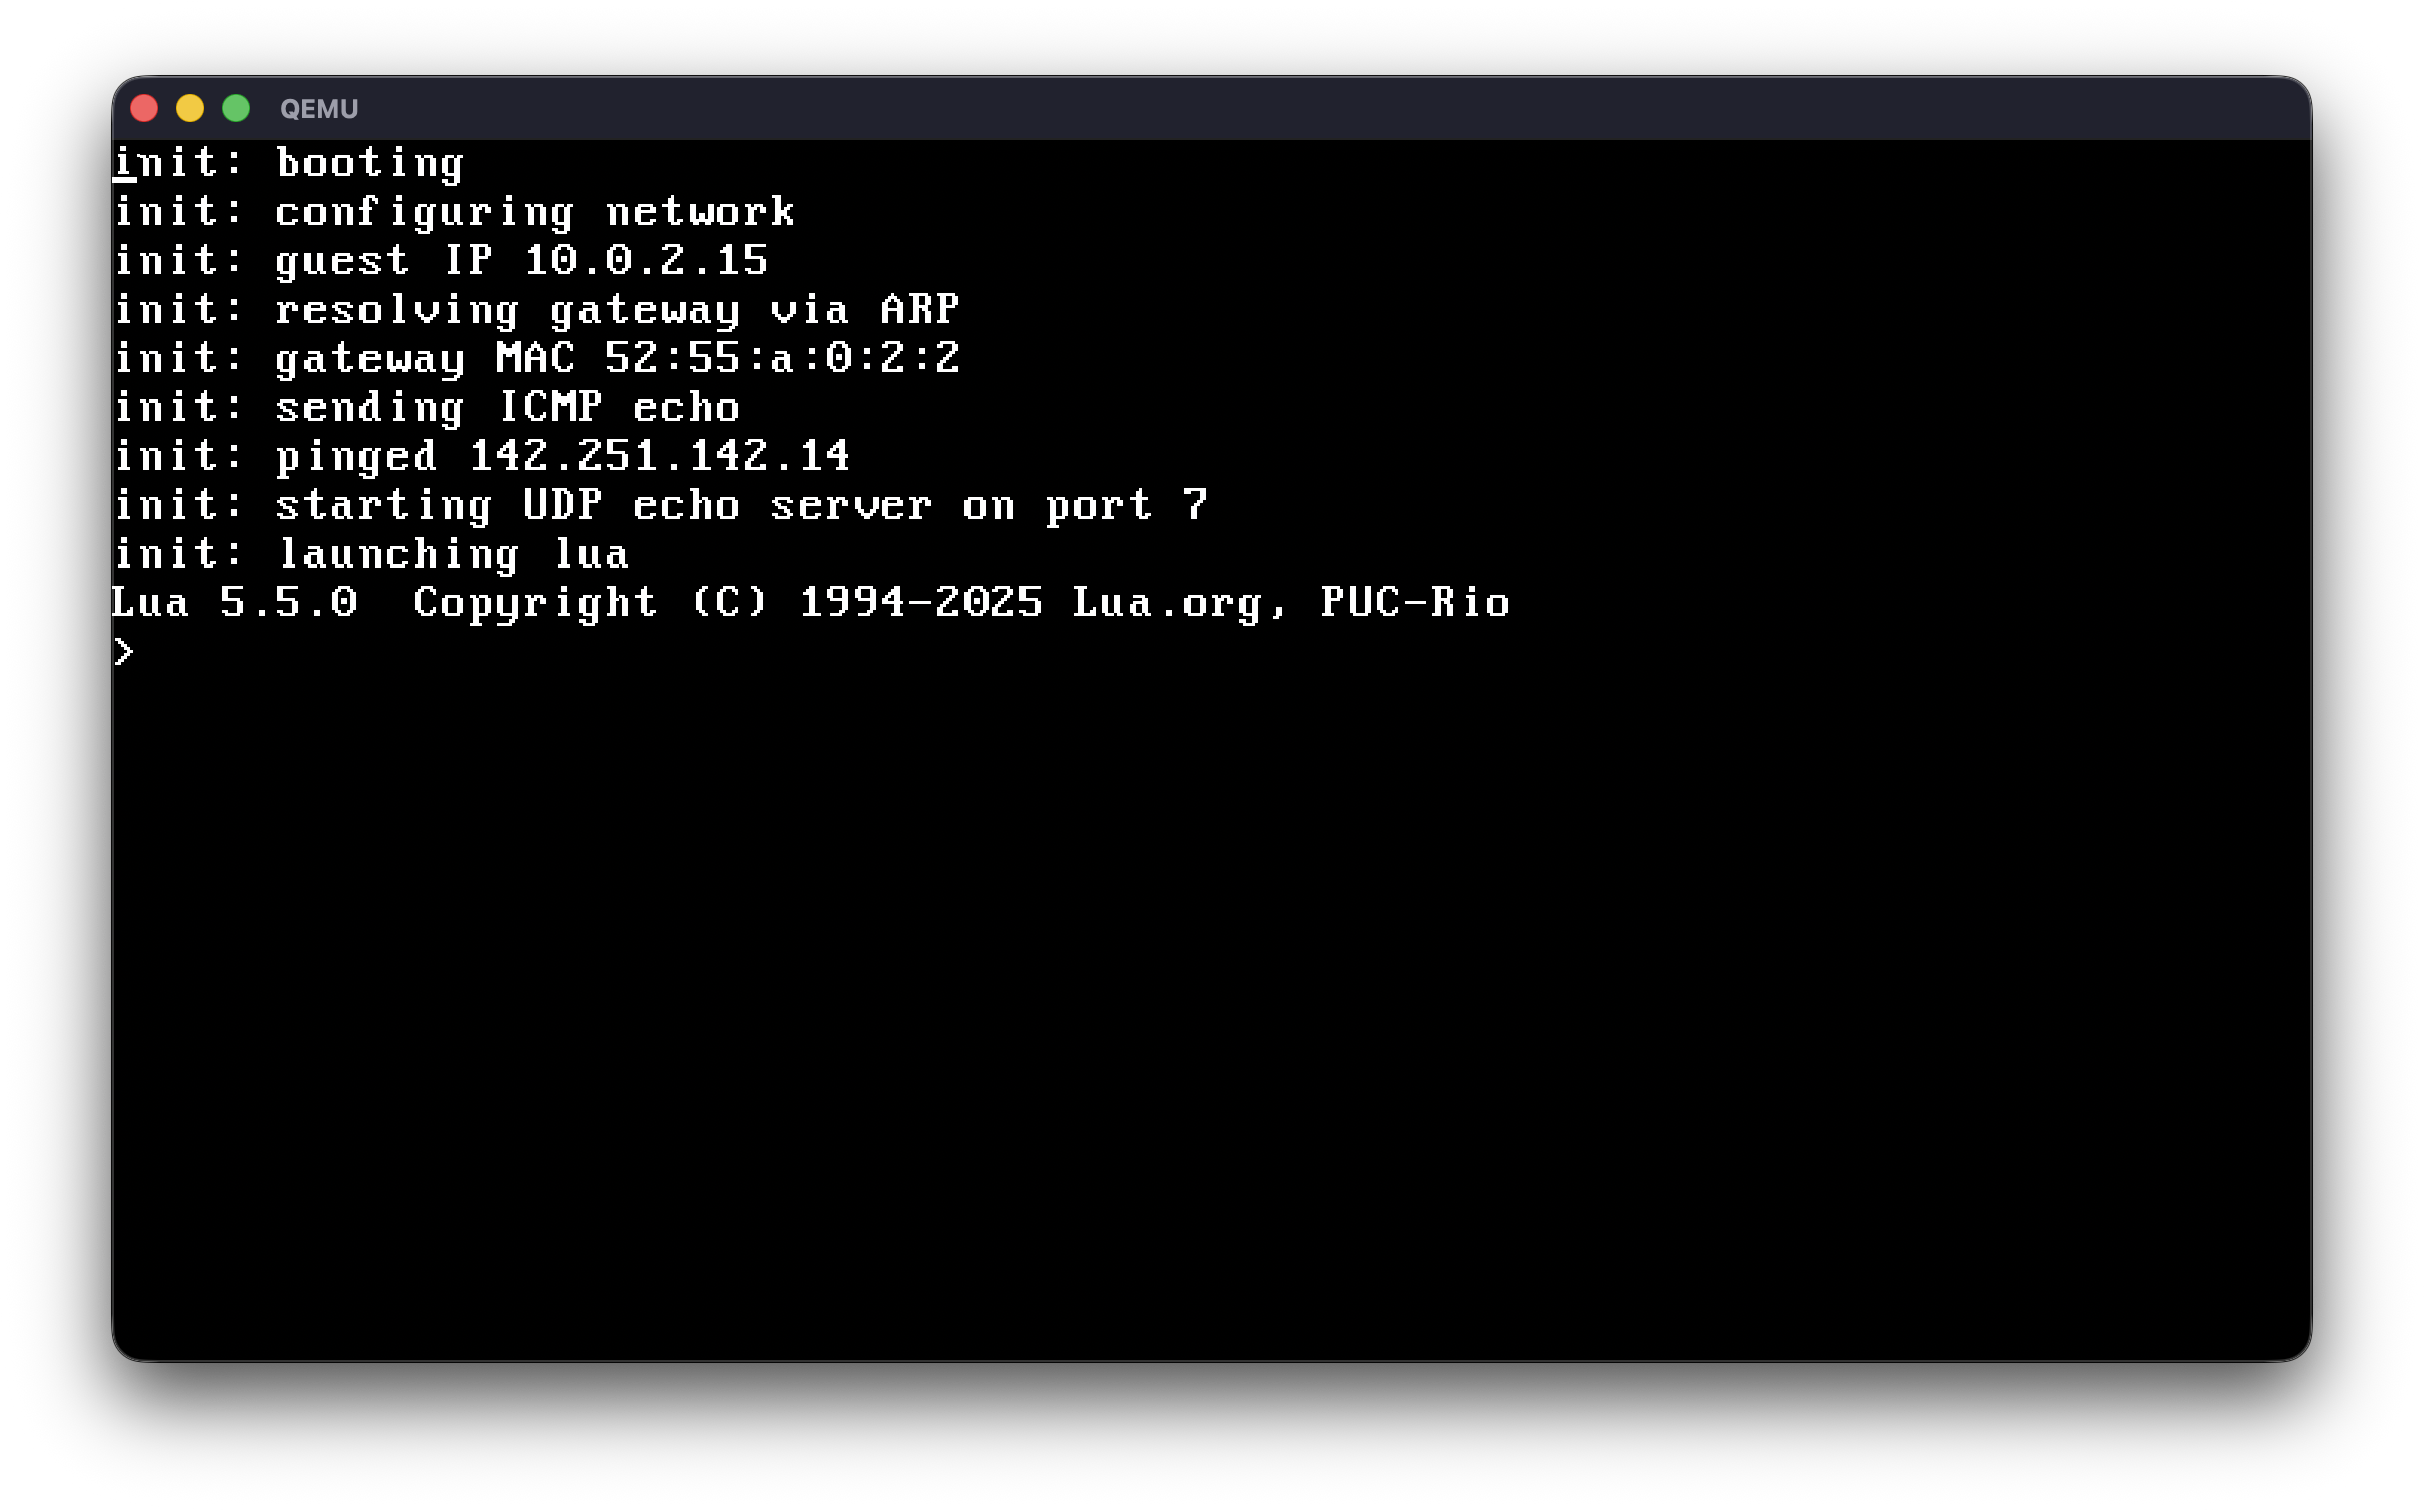
\includegraphics[width=0.9\textwidth]{mboot_init.png}
\caption{The mboot console (QEMU, VGA text mode) after boot, from the
August 2026 build. \texttt{init}
brings up the network: it resolves the gateway via ARP, sends an ICMP echo
to a public host, and starts a UDP echo server on port 7. It then
launches Lua 5.5.0, leaving an interactive prompt. (The init system has
since been simplified; see Section~\ref{sec:testing}.)}
\label{fig:init}
\end{figure}

\begin{figure}[htbp]
\centering
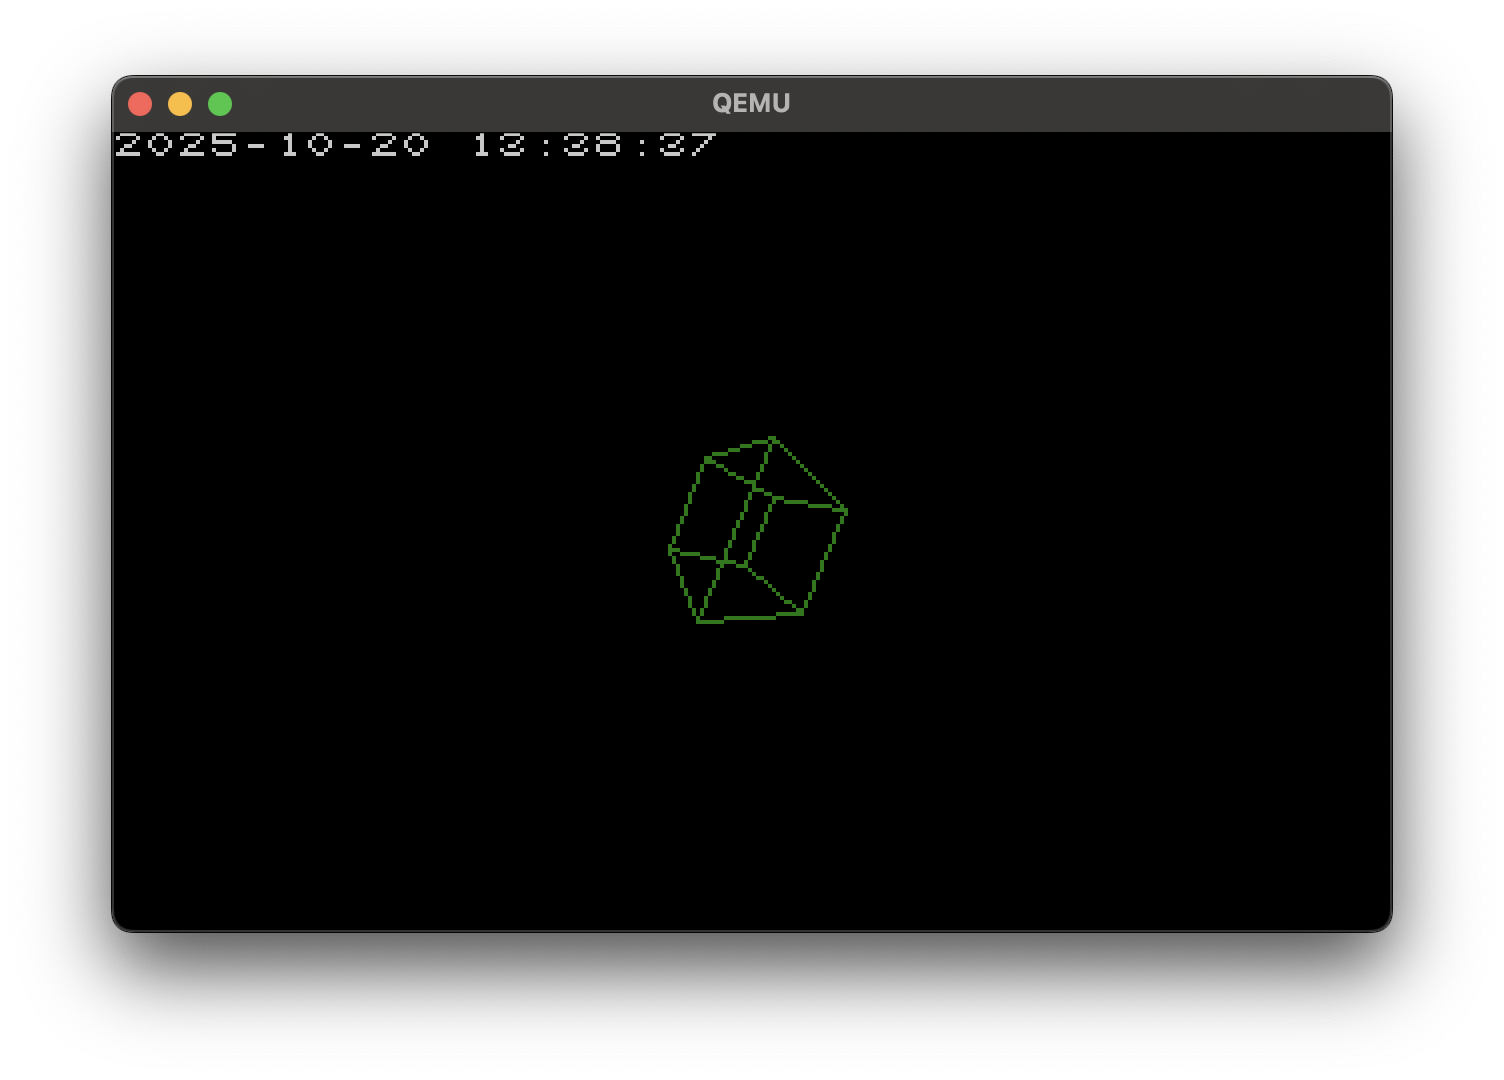
\includegraphics[width=0.9\textwidth]{mboot_cube_time.png}
\caption{A more demanding Lua workload: a wireframe cube and a timestamp
rendered to the VGA console from inside the Lua REPL.}
\label{fig:cube}
\end{figure}

The fact that Lua 5.5.0 runs successfully demonstrates that the operating
system provides all the infrastructure that a real language runtime
needs: memory allocation, file I/O, process management, a C library, and
a working interrupt and timer system. That was the goal I set in
Section~\ref{sec:goals}, and it is met.

\section{Reflection and What I Learned}
\label{sec:reflection}

What I take away from the project sits on three levels. The obvious one
is subject matter: I now know how a boot flow works end to end, how the
CPU switches between privilege levels, how paging provides memory
isolation, and how a scheduler juggles several tasks, knowledge I got
by reading the Intel SDM, writing the assembly, and debugging all of it
without a safety net.

The second level is process. Managing a project that grew from a few
hundred lines to several thousand forced me to read code I did not write
(the Lua source, datasheets, RFCs) and pull out what mattered. It
also forced me to plan in layers, and to change the plan without
pretending the old one had been right all along.

Third, and least fun: debugging is a skill. My first sessions were
hours of flailing at symptoms. Near the end I could usually go from a
crash to the guilty subsystem in an afternoon, mostly by resisting the
urge to change three things at once.

On scope I did badly and know it. The scheduler, the TTYs, and the VFS
layer grew past the original design and all three earned their keep:
without them there is one Lua prompt, not four. The network stack never
earned anything back: nothing in it was needed to run Lua, and it is
where most of my scope drift came from. If I started over I would defend
the core goal harder and let the network stack stay an experiment.

The last thing worth saying is smaller: writing an operating system is
hard but achievable. There is no trick to it beyond building
incrementally, testing constantly, and being willing to delete code that
does not work, which, inconveniently, is also the boring advice.

\section{Conclusion}
\label{sec:conclusion}

I set out to build an operating system capable of running Lua 5.5.0. I
planned it as a layered system, built it one subsystem at a time, and
debugged it using QEMU, serial output, and GDB. The final system boots
from BIOS, loads user programs from a FAT16 disk, and runs Lua 5.5.0 as
a user program. It includes a preemptive scheduler, paging, a VFS layer,
a VGA console, a serial port, a PCI bus driver, an e1000 network driver,
and a small network stack.

The project was difficult, and not only in the places I expected. Bugs
appeared in the bootloader, the memory allocator, the paging system, the
scheduler, and the C library; two designs I was confident in (the PIE
plan, the first scheduler) had to be thrown out; and filesystem write
support and a complete C library never made it past the deadline.

It works the way I hoped, though: Lua 5.5.0 runs on an
OS I wrote from scratch. Four terminals, each with a live Lua prompt,
switching between them with Alt+F1 through Alt+F4. That is the image
I will remember, because it is the moment the scheduler stopped being a
diagram and started being real.

If I were to continue the project, I would add filesystem write support,
proper memory management with \texttt{sbrk} and \texttt{mmap}, and a more
complete C library. I would also add user-mode privilege separation and
SMP support. Neither is needed for the goal I set, though: as it stands,
\texttt{mboot} is a small operating system that runs a real language
runtime, and I built it from scratch.

\section*{References}
\phantomsection
\label{sec:refs}
\addcontentsline{toc}{section}{References}

\begin{enumerate}[nosep, label={[\arabic*]}]
  \item Intel Corporation. \emph{Intel 64 and IA-32 Architectures Software
  Developer's Manual, Volume 3A: System Programming Guide, Part 1.}
  \url{https://www.intel.com/content/www/us/en/developer/articles/technical/intel-sdm.html}
  \item OSDev Wiki. \emph{Bare Bones, GDT, IDT, Paging, Detecting Memory
  (E820), PIC, PIT, PS/2 Keyboard, VGA Hardware, Serial Ports, ATA PIO
  Mode, FAT, ELF, PCI, Lua.} \url{https://wiki.osdev.org/}
  \item Microsoft Corporation. \emph{Microsoft Extensible Firmware
  Initiative FAT32 File System Specification, v1.03.}
  \url{https://academy.cba.mit.edu/classes/networking_communications/SD/FAT.pdf}
  \item Tool Interface Standard. \emph{Executable and Linkable Format
  (ELF) Specification, Version 1.2.}
  \url{https://refspecs.linuxfoundation.org/elf/elf.pdf}
  \item J.~Postel. \emph{RFC 791: Internet Protocol.} IETF, 1981.
  \url{https://datatracker.ietf.org/doc/html/rfc791}
  \item D.~Plummer. \emph{RFC 826: An Ethernet Address Resolution
  Protocol.} IETF, 1982.
  \url{https://datatracker.ietf.org/doc/html/rfc826}
  \item J.~Postel. \emph{RFC 768: User Datagram Protocol.} IETF, 1980.
  \url{https://datatracker.ietf.org/doc/html/rfc768}
  \item J.~Postel. \emph{RFC 792: Internet Control Message Protocol.}
  IETF, 1981. \url{https://datatracker.ietf.org/doc/html/rfc792}
  \item Intel Corporation. \emph{PCI/PCI-X Family of Gigabit Ethernet
  Controllers Software Developer's Manual (82540EM / 82574L).}
  \url{https://www.intel.com/content/dam/www/public/us/en/documents/manuals/gigabit-ethernet-controller-datasheet.pdf}
  \item R.~Ierusalimschy, L.~H.~de~Figueiredo, and W.~Filho. \emph{Lua 5.5
  Reference Manual.} PUC-Rio, 2025. \url{https://www.lua.org/manual/5.5/}
  \item The Lua Team. \emph{Lua 5.5.0 source code.}
  \url{https://www.lua.org/ftp/lua-5.5.0.tar.gz}
  \item QEMU Project. \emph{QEMU System Emulation Documentation.}
  \url{https://www.qemu.org/docs/master/system/}
\end{enumerate}

\end{document}
